%
% HR.tex
% Human Resources
%
% Aleph Objects Operations Manual
%
% Copyright (C) 2014, 2015 Aleph Objects, Inc.
%
% This document is licensed under the Creative Commons Attribution 4.0
% International Public License (CC BY-SA 4.0) by Aleph Objects, Inc.
%

\input{HR-jobs}

\section{Professional Employment Organizations (PEO)}
Insperity.

\section{Employee Benefits}
See employee handbook at \texttt{http://esc.insperitiy.com}

\section{Logging hours in OpenERP}
For hourly Insperity employees:

OpenERP ---> Human Resources ---> Attendences ---> Attendences

For hourly Kelly employees, track your hours on Kelly's website.

\section{Requesting time off in OpenERP}
OpenERP ---> Human Resources ---> Leaves ---> Leave Requests

\section{Recruitment / Interviewing}
Kelly, Insperity, JobZology.

\section{Performance}
Insperity.

\section{Training}
Certifications.

\section{Organizational Chart}
See figure \ref{fig:ao_org_chart} for Aleph Object's organizational chart.
\input{OrgChart}

See figure \ref{fig:ao_org_chart_dot} for Aleph Object's organizational chart in dot.

\begin{sidewaysfigure}[p]
\thisfloatpagestyle{empty}
% The ao-orgchart-dot.png was built in dot.
\includegraphics[keepaspectratio=true,height=1.10\textheight,width=1.00\textwidth,angle=-90]{ao-orgchart-dot.png}
 \caption{Aleph Objects Org Chart dot}
 \label{fig:ao_org_chart_dot}
\end{sidewaysfigure}

\section{Schedules}
The following calendars list when there are recurring meetings.

%
% SchedWeek.tex
% Weekly Recurring Events Schedule
%
% Aleph Objects Operations Manual
%
% Copyright (C) 2014, 2015 Aleph Objects, Inc.
%
% This document is licensed under the Creative Commons Attribution 4.0
% International Public License (CC BY-SA 4.0) by Aleph Objects, Inc.
%

% Be sure to set the timestamp below, which prints the version number on the
% document, so it is easy to see if it is the latest version when printed out.

% These set the width of a day and the height of an hour.
\newcommand*\daywidth{3.7cm}
\newcommand*\hourheight{3.8em}

% The entry style will have two options:
% * the first option sets how many hours the entry will be (i.e. its height);
% * the second option sets how many overlapping entries there are (thus
%   determining the width).
\tikzset{entry/.style 2 args={
    xshift=(0.5334em+0.8pt)/2,
    draw,
    line width=0.8pt,
    font=\sffamily,
    rectangle,
    rounded corners,
    fill=blue!20,
    anchor=north west,
    inner sep=0.3333em,
    text width={\daywidth/#2-1.2em-1.6pt},
    minimum height=#1*\hourheight,
    align=center
}}

% Start the picture and set the x coordinate to correspond to days and the y
% coordinate to correspond to hours (y should point downwards).
\begin{sidewaysfigure}[p]
\thisfloatpagestyle{empty}
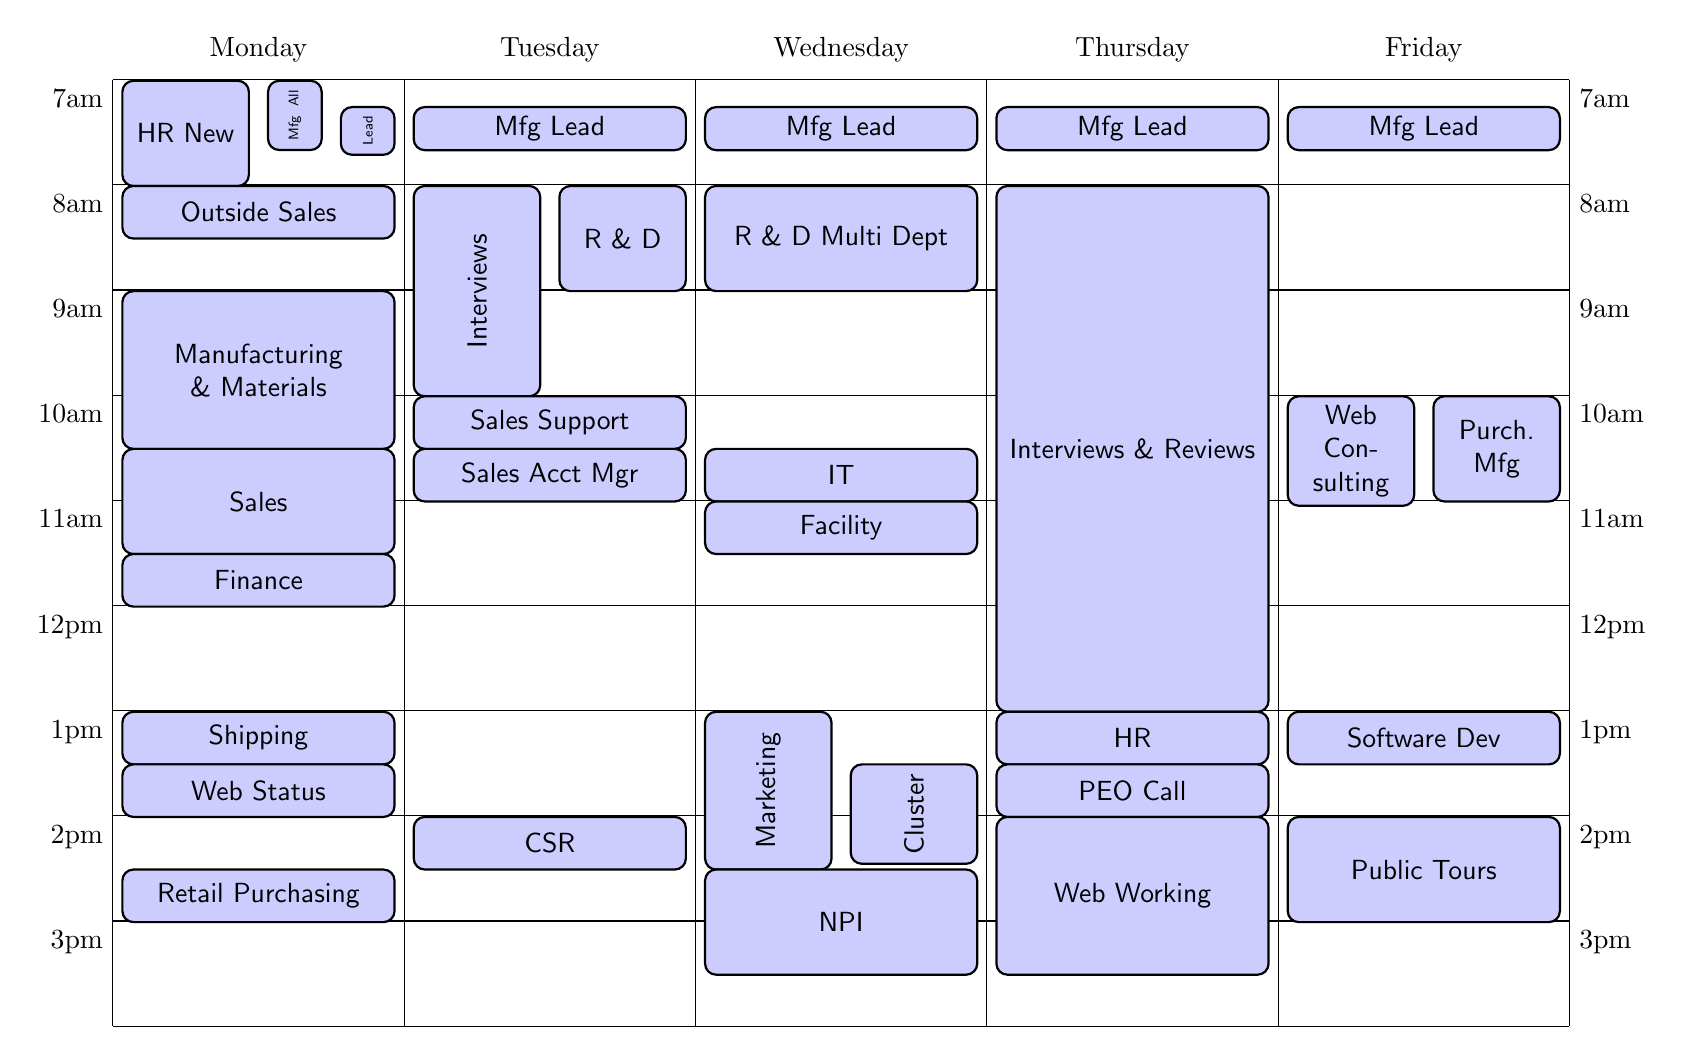
\begin{tikzpicture}[y=-\hourheight,x=\daywidth]

    % First print a list of times.
    \foreach \time/\ustime in {7/7am,8/8am,9/9am,10/10am,11/11am,12/12pm,13/1pm,14/2pm,15/3pm}
        \node[anchor=north east] at (1,\time) {\ustime};

    % Draw some day dividers.
    \draw (1,7) -- (1,16);
    \draw (2,7) -- (2,16);
    \draw (3,7) -- (3,16);
    \draw (4,7) -- (4,16);
    \draw (5,7) -- (5,16);
    \draw (6,7) -- (6,16);
    
    % Draw some hour dividers.
    \draw (1,7) -- (6,7);
    \draw (1,8) -- (6,8);
    \draw (1,9) -- (6,9);
    \draw (1,10) -- (6,10);
    \draw (1,11) -- (6,11);
    \draw (1,12) -- (6,12);
    \draw (1,13) -- (6,13);
    \draw (1,14) -- (6,14);
    \draw (1,15) -- (6,15);
    \draw (1,16) -- (6,16);

    \foreach \time/\ustime in {7/7am,8/8am,9/9am,10/10am,11/11am,12/12pm,13/1pm,14/2pm,15/3pm}
        \node[anchor=north west] at (6,\time) {\ustime};
        
    % Start Monday.
    % Write the entries. Note that the x coordinate is 1 (for Monday) plus an
    % appropriate amount of shifting. The y coordinate is simply the starting
    % time.
    % 1=Monday, 2=Tuesday, 3=Wednesday, 4=Thursday, 5=Friday
    %\node[entry={DURATION}{COLUMN WIDTH?}] at (DAY,HOUR) {TEXT};

    % Monday
    \node[anchor=north] at (1.5,6.5) {Monday};
    \node[entry={1.0}{2}] at (1,7) {HR New};
    \node[entry={0.25}{4}] at (1.5,7)  {\rotatebox{90}{\tiny{Mfg All}}};
    \node[entry={0.25}{4}] at (1.75,7.25)  {\rotatebox{90}{\tiny{Lead}}};
    \node[entry={0.5}{1}] at (1,8) {Outside Sales};
    \node[entry={1.5}{1}] at (1,9) {Manufacturing \& Materials};
    \node[entry={1.0}{1}] at (1,10.5){Sales};
    \node[entry={0.5}{1}] at (1,11.5) {Finance};
    \node[entry={0.5}{1}] at (1,13) {Shipping};
    \node[entry={0.5}{1}] at (1,13.5) {Web Status};
    \node[entry={0.5}{1}] at (1,14.5) {Retail Purchasing};

    % Tuesday
    \node[anchor=north] at (2.5,6.5) {Tuesday};
    \node[entry={0.25}{1}] at (2,7.25) {Mfg Lead};
    \node[entry={2.0}{2}] at (2,8) {\rotatebox{90}{Interviews}};
    \node[entry={1.0}{2}] at (2.5,8) {R \& D};
    \node[entry={0.5}{1}] at (2,10) {Sales Support};
    \node[entry={0.5}{1}] at (2,10.5) {Sales Acct Mgr};
    \node[entry={0.5}{1}] at (2,14) {CSR};
    
    % Wednesday
    \node[anchor=north] at (3.5,6.5) {Wednesday};
    \node[entry={0.25}{1}] at (3,7.25) {Mfg Lead};
    \node[entry={1.0}{1}] at (3,8) {R \& D Multi Dept};
    \node[entry={0.5}{1}] at (3,10.5) {IT};
    \node[entry={0.5}{1}] at (3,11) {Facility};
    \node[entry={1.5}{2}] at (3,13) {\rotatebox{90}{Marketing}};
    \node[entry={0.5}{2}] at (3.5,13.5) {\rotatebox{90}{Cluster}};
    \node[entry={1.0}{1}] at (3,14.5) {NPI};
    
    % Thursday
    \node[anchor=north] at (4.5,6.5) {Thursday};
    \node[entry={0.25}{1}] at (4,7.25) {Mfg Lead};
    \node[entry={5.0}{1}] at (4,8) {Interviews \& Reviews};
    \node[entry={0.5}{1}] at (4,13) {HR};
    \node[entry={0.5}{1}] at (4,13.5) {PEO Call};
    \node[entry={1.5}{1}] at (4,14) {Web Working};
    
    % Friday
    \node[anchor=north] at (5.5,6.5) {Friday};
    \node[entry={0.25}{1}] at (5,7.25) {Mfg Lead};
    \node[entry={1.0}{2}] at (5,10) {Web Consulting};
    \node[entry={1.0}{2}] at (5.5,10) {Purch. Mfg};
    \node[entry={0.5}{1}] at (5,13) {Software Dev};
    \node[entry={1.0}{1}] at (5,14) {Public Tours};

\end{tikzpicture}
\caption{Weekly Company Meetings, Day Shift}
\renewcommand{\dateseparator}{}
% Timestamp Version: YYYY-MM-DD-Serial
\hfill\texttt{v.2015-07-07-1}

 \label{fig:ao_week_meet}
\end{sidewaysfigure}


See figure \ref{fig:ao_week_meet} for Aleph Object's weekly meeting schedule, day shift.
%
% SchedWeekEvening.tex
% Weekly Recurring Events Schedule, Evening Shift
%
% Aleph Objects Operations Manual
%
% Copyright (C) 2014, 2015 Aleph Objects, Inc.
%
% This document is licensed under the Creative Commons Attribution 4.0
% International Public License (CC BY-SA 4.0) by Aleph Objects, Inc.
%

% Be sure to set the timestamp below, which prints the version number on the
% document, so it is easy to see if it is the latest version when printed out.

% These set the width of a day and the height of an hour.
\renewcommand*\daywidth{3.7cm}
\renewcommand*\hourheight{3.8em}

% The entry style will have two options:
% * the first option sets how many hours the entry will be (i.e. its height);
% * the second option sets how many overlapping entries there are (thus
%   determining the width).
\tikzset{entry/.style 2 args={
    xshift=(0.5334em+0.8pt)/2,
    draw,
    line width=0.8pt,
    font=\sffamily,
    rectangle,
    rounded corners,
    fill=blue!20,
    anchor=north west,
    inner sep=0.3333em,
    text width={\daywidth/#2-1.2em-1.6pt},
    minimum height=#1*\hourheight,
    align=center
}}

% Start the picture and set the x coordinate to correspond to days and the y
% coordinate to correspond to hours (y should point downwards).
\begin{sidewaysfigure}[p]
\thisfloatpagestyle{empty}
\begin{tikzpicture}[y=-\hourheight,x=\daywidth]

    % First print a list of times.
    \foreach \time/\ustime in {16/4pm,17/5pm,18/6pm,19/7pm,20/8pm,21/9pm,22/10pm,23/11pm}
        \node[anchor=north east] at (1,\time) {\ustime};

    % Draw some day dividers.
    \draw (1,16) -- (1,24);
    \draw (2,16) -- (2,24);
    \draw (3,16) -- (3,24);
    \draw (4,16) -- (4,24);
    \draw (5,16) -- (5,24);
    \draw (6,16) -- (6,24);
    \draw (7,16) -- (7,24);
    \draw (7,16) -- (7,24);
    
    % Draw some hour dividers.
    \draw (1,16) -- (6,16);
    \draw (1,17) -- (6,17);
    \draw (1,18) -- (6,18);
    \draw (1,19) -- (6,19);
    \draw (1,20) -- (6,20);
    \draw (1,21) -- (6,21);
    \draw (1,22) -- (6,22);
    \draw (1,23) -- (6,23);
    \draw (1,24) -- (6,24);

    \foreach \time/\ustime in {16/4pm,17/5pm,18/6pm,19/7pm,20/8pm,21/9pm,22/10pm,23/11pm}
        \node[anchor=north west] at (6,\time) {\ustime};
        
    % Start Monday.
    % Write the entries. Note that the x coordinate is 1 (for Monday) plus an
    % appropriate amount of shifting. The y coordinate is simply the starting
    % time.
    % 1=Monday, 2=Tuesday, 3=Wednesday, 4=Thursday, 5=Friday
    %\node[entry={DURATION}{COLUMN WIDTH?}] at (DAY,HOUR) {TEXT};

    % Monday
    \node[anchor=north] at (1.5,15) {Monday};

    % Tuesday
    \node[anchor=north] at (2.5,15) {Tuesday};
    
    % Wednesday
    \node[anchor=north] at (3.5,15) {Wednesday};
    
    % Thursday
    \node[anchor=north] at (4.5,15) {Thursday};
    
    % Friday
    \node[anchor=north] at (5.5,15) {Friday};

\end{tikzpicture}
\caption{Weekly Company Meetings, Evening Shift}
\renewcommand{\dateseparator}{}
% Timestamp Version: YYYY-MM-DD-Serial
\hfill\texttt{v.2015-07-07-1}

 \label{fig:ao_week_meet_night}
\end{sidewaysfigure}


See figure \ref{fig:ao_week_meet_evening} for Aleph Object's weekly meeting schedule, evening shift.
%
% SchedWeekNight.tex
% Weekly Recurring Events Schedule, Night Shift
%
% Aleph Objects Operations Manual
%
% Copyright (C) 2014, 2015 Aleph Objects, Inc.
%
% This document is licensed under the Creative Commons Attribution 4.0
% International Public License (CC BY-SA 4.0) by Aleph Objects, Inc.
%

% Be sure to set the timestamp below, which prints the version number on the
% document, so it is easy to see if it is the latest version when printed out.

% These set the width of a day and the height of an hour.
\renewcommand*\daywidth{3.7cm}
\renewcommand*\hourheight{3.8em}

% The entry style will have two options:
% * the first option sets how many hours the entry will be (i.e. its height);
% * the second option sets how many overlapping entries there are (thus
%   determining the width).
\tikzset{entry/.style 2 args={
    xshift=(0.5334em+0.8pt)/2,
    draw,
    line width=0.8pt,
    font=\sffamily,
    rectangle,
    rounded corners,
    fill=blue!20,
    anchor=north west,
    inner sep=0.3333em,
    text width={\daywidth/#2-1.2em-1.6pt},
    minimum height=#1*\hourheight,
    align=center
}}

% Start the picture and set the x coordinate to correspond to days and the y
% coordinate to correspond to hours (y should point downwards).
\begin{sidewaysfigure}[p]
\thisfloatpagestyle{empty}
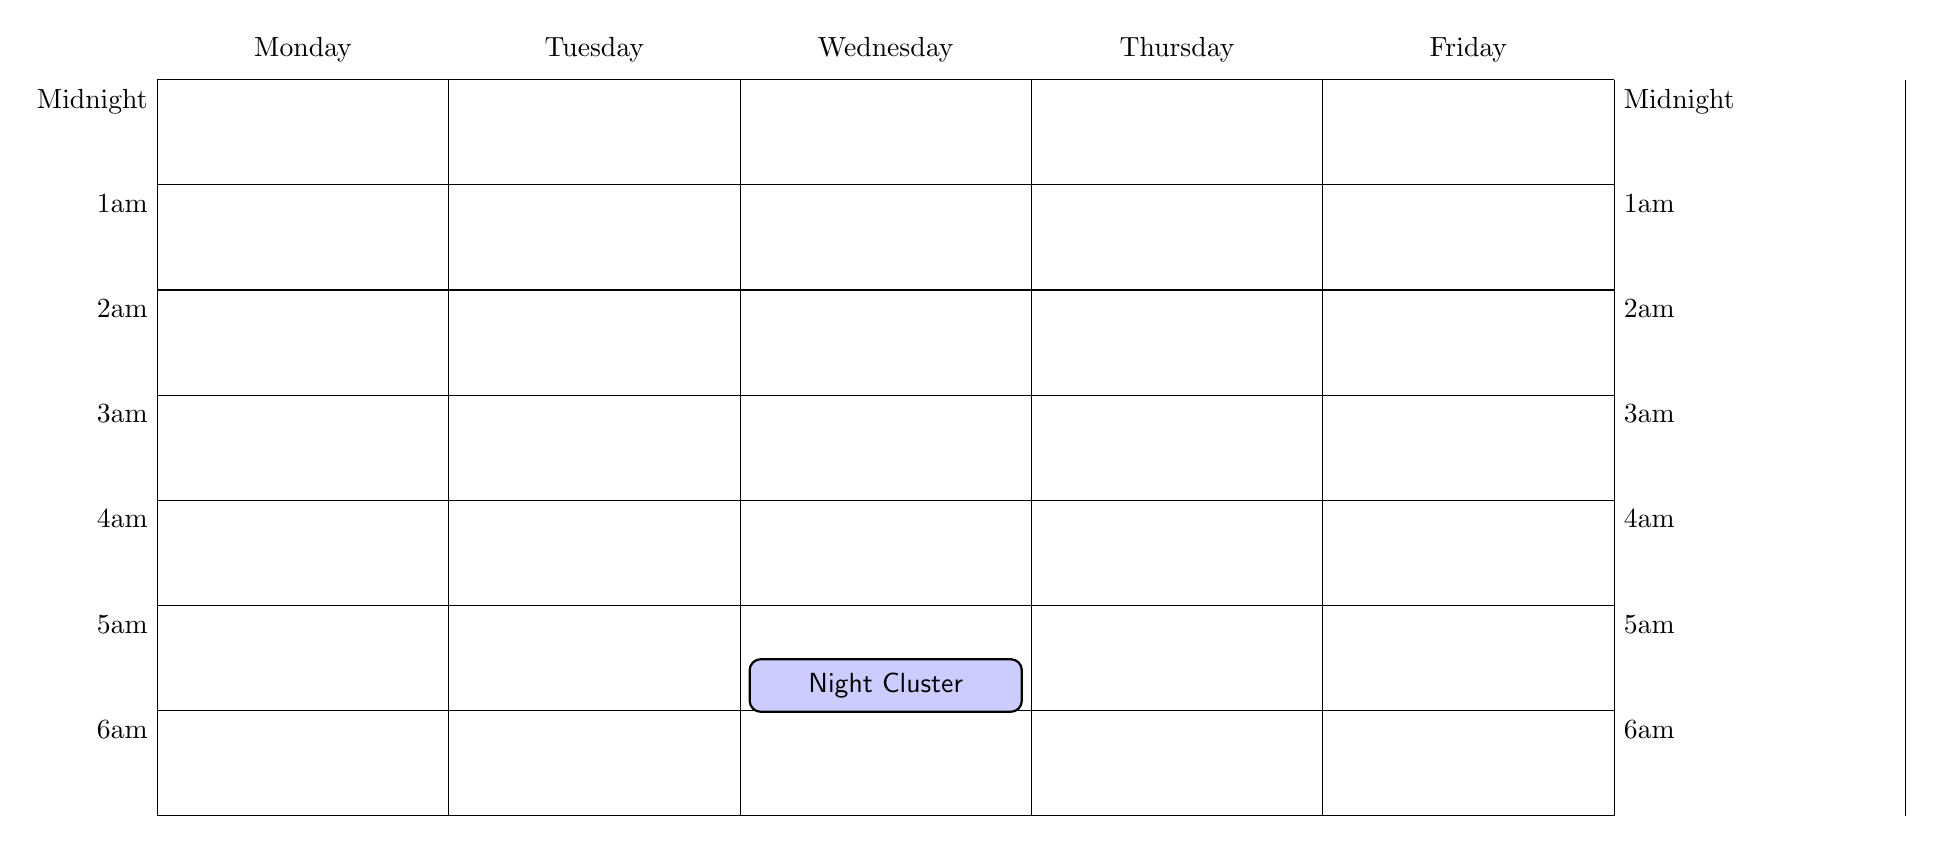
\begin{tikzpicture}[y=-\hourheight,x=\daywidth]

    % First print a list of times.
    \foreach \time/\ustime in {0/Midnight,1/1am,2/2am,3/3am,4/4am,5/5am,6/6am}
        \node[anchor=north east] at (1,\time) {\ustime};

    % Draw some day dividers.
    \draw (1,0) -- (1,7);
    \draw (2,0) -- (2,7);
    \draw (3,0) -- (3,7);
    \draw (4,0) -- (4,7);
    \draw (5,0) -- (5,7);
    \draw (6,0) -- (6,7);
    \draw (7,0) -- (7,7);
    
    % Draw some hour dividers.
    \draw (1,0) -- (6,0);
    \draw (1,1) -- (6,1);
    \draw (1,2) -- (6,2);
    \draw (1,3) -- (6,3);
    \draw (1,4) -- (6,4);
    \draw (1,5) -- (6,5);
    \draw (1,6) -- (6,6);
    \draw (1,7) -- (6,7);

    \foreach \time/\ustime in {0/Midnight,1/1am,2/2am,3/3am,4/4am,5/5am,6/6am}
        \node[anchor=north west] at (6,\time) {\ustime};
        
    % Start Monday.
    % Write the entries. Note that the x coordinate is 1 (for Monday) plus an
    % appropriate amount of shifting. The y coordinate is simply the starting
    % time.
    % 1=Monday, 2=Tuesday, 3=Wednesday, 4=Thursday, 5=Friday
    %\node[entry={DURATION}{COLUMN WIDTH?}] at (DAY,HOUR) {TEXT};

    % Monday
    \node[anchor=north] at (1.5,-0.5) {Monday};

    % Tuesday
    \node[anchor=north] at (2.5,-0.5) {Tuesday};
    
    % Wednesday
    \node[anchor=north] at (3.5,-0.5) {Wednesday};
    \node[entry={0.5}{1}] at (3,5.5) {Night Cluster};
    
    % Thursday
    \node[anchor=north] at (4.5,-0.5) {Thursday};
    
    % Friday
    \node[anchor=north] at (5.5,-0.5) {Friday};

\end{tikzpicture}
\caption{Weekly Company Meetings, Night Shift}
\renewcommand{\dateseparator}{}
% Timestamp Version: YYYY-MM-DD-Serial
\hfill\texttt{v.2015-07-07-1}

 \label{fig:ao_week_meet_night}
\end{sidewaysfigure}


See figure \ref{fig:ao_week_meet_night} for Aleph Object's weekly meeting schedule, night shift.
\input{SchedMonth}
See figure \ref{fig:ao_month_meet} for Aleph Object's monthly company meeting schedule.
